% !TeX program = lualatex -synctex=1 -interaction=nonstopmode --shell-escape %.tex

\documentclass[_Venture_p3.tex]{subfiles}

\begin{document}

\setbeamercovered{invisible}

\subsection{Сущность подрывных инноваций}
\begin{frame}[shrink=5]{Сущность подрывных инноваций}
\begin{itemize}
	\item компании-лидеры обычно создают новые продукты и услуги в таком темпе, который превосходит темп ``усвоения`` этих инноваций;
	\item все ``подрывные`` продукты создаются с расчетом на такие возможности роста, которые находятся вне ядерных рынков лидера.
\end{itemize}
\end{frame}


\begin{frame}{Сущность подрывных инноваций}
\begin{figure}
	\centering
	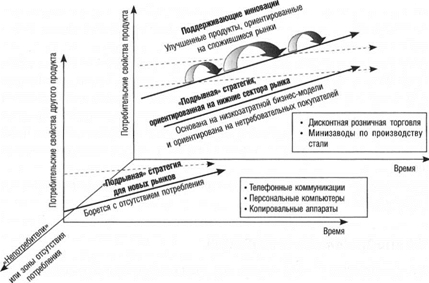
\includegraphics[scale=.8]{img/disruptive_innovations_strategy}
	\caption{Стратегия компании создающей подрывные инновации}
\end{figure}
\end{frame}

\begin{frame}{Типы подрывных продуктов}
\begin{itemize}
	\item продукты, ориентированные на новые рынки: конкуренция с отсутствием потребления и создание совершенно нового рынка;
	\item продукты, ориентированные на нижние сектора рынка: бизнес-модель, которая позволит с прибылью для себя обслуживать наименее взыскательных потребителей. Лидеры рынка с радостью отказываются от таких потребителей, поскольку сами стремятся продвигаться в более высокие сектора рынка.
\end{itemize}
\end{frame}

\subsection{Концепция ресурсов, процедур и ценностей}
\begin{frame}{Концепция ресурсов, процедур и ценностей (РПЦ)}
\begin{table}
	\centering
	\scriptsize
	% Table generated by Excel2LaTeX from sheet 'Лист1'
	\begin{table}[htbp]
		\centering
		\caption{\captionf{Концепция ресурсов,\\ процедур и ценностей (РПЦ)}}
		\begin{tabularx}{\linewidth}[b]
			{@{}>{\raggedright\arraybackslash}XXX@{}}
			%\setrulecolor
			\setrulecolor\toprule
			\cnamef{Ресурсы} & \cnamef{Процедуры} & \cnamef{Ценности} \\\midrule
			Продукция и активы & Схемы работы & Критерии приоритетов \\
			Персонал &  Прием на работу и обучение &  Структура издержек \\
			Технологии &  Разработка продуктов &  Финансовый отчет \\
			Продукты &  Производство &  Потребности покупателей \\
			Оборудование &  Бюджет и планирование &  Критерии перспективных возможностей \\
			Информация &  Исследование рынка &  Этические принципы \\
			Денежные средства &  Процесс распределения ресурсов &  \\
			Бренды &       &  \\
			Каналы реализации &       &  \\
			\bottomrule
		\end{tabularx}%
		\label{tab:addlabel}%
	\end{table}%
\end{table}
\end{frame}

\begin{frame}
Концепция РПЦ утверждает, что организация может успешно использовать открывающиеся возможности только тогда, когда у нее имеются необходимые ресурсы, когда процедуры способствуют, а не препятствуют необходимым действиям; и когда корпоративные ценности позволяют присвоить перспективному проекту более высокую приоритетность по сравнению с прочими проектами, претендующими на корпоративные ресурсы. 
\end{frame}

\begin{frame}
Компании-лидеры хорошо продвигают поддерживающие инновации, потому что именно такие инновации становятся приоритетными в соответствии с ценностями этих компаний. К тому же процедуры и ресурсы этих компаний организованы в точности так, как нужно для обслуживания поддерживающих инноваций. Однако лидеры рынка терпят крах, когда конкурируют с теми, кто продвигает «подрывные» инновации.
\end{frame}

\subsection{Концепция ``найма продуктов на работу``}
\begin{frame}{Концепция ``найма продуктов на работу``	}
\begin{itemize}
	\small
	\item Приобретая тот или иной продукт, потребитель на самом деле ``платит про­дукту зарплату``, с тем чтобы он выполнял определенные ``поручения`` своего хозяина.
	\item Компания добивается успеха, когда ее продукты позволяют потребителям с большим комфортом делать то, что для них всегда имело значение.
	\item Компании считают, что если продукт удовлетворяет потребности определенного сегмента рынка, то этот продукт будет успешным. 
\end{itemize}
\end{frame}

\begin{frame}{Ложные схемы сегментации рынка }{основная причина поразительно большого числа неудач при разработке новых продуктов}
\begin{itemize}
	\small
	\item Продукты,  соответствующие определенной жизненной ситуации потребления, в конце концов и оказываются настоящими лидерами продаж. Такие про­дукты позволяют потребителю благополучно делать то, что он уже пытался делать и прежде, но с меньшим успехом.
	\item Выяснив, какие именно виды ``заданий`` действительно имеют значение для наших потребителей, можно разработать продукты, которые будут легко справляться с такой ``работой``. Таким образом, компания обнаружит новые рынки, о существовании которых до тех пор никто даже и не подозревал. 
\end{itemize}
\end{frame}

\subsection{Концепция развития цепочки создания стоимости (РЦСС)}
\begin{frame}{Концепция развития цепочки создания стоимости (РЦСС)}
\begin{figure}
	\centering
	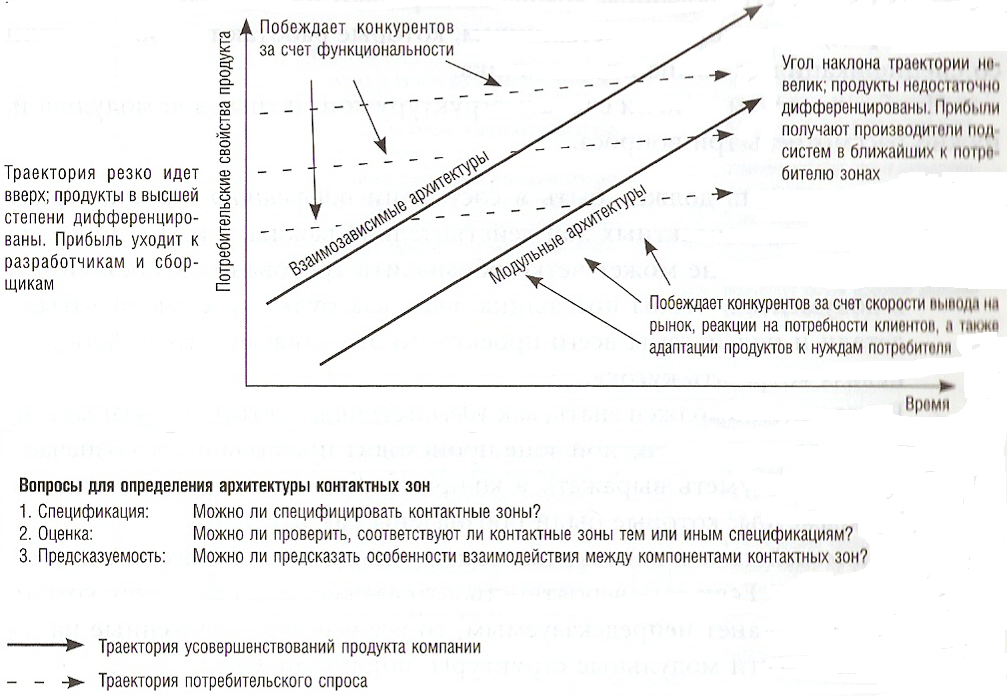
\includegraphics[scale=.4]{img/value_chain_development}
	\caption{Развитие цепочки создания стоимости }
\end{figure}
\end{frame}


\begin{frame}
Обычно отрасль в своем развития переходит от стадии господства взаимозави­симой архитектуры, когда ведущие компании должны идти на вертикальную интеграцию, к стадии модульности, когда самая большая доля добавленной стоимости производится специализированными компаниями, отвечающими за жизненно важные зоны цепочки создания стоимости и выпускающими самые важные детали и подсистемы.
\end{frame}

\begin{frame}
\begin{itemize}
	\small
	\item Когда качество продукта еще не соответствует требованиям основного направления рынка, именно интегрированные компании получают конкурентные преимущества. 
	\item Такие компании лучше других умеют справляться с теми сложностями, которые возникают при разработке усовершенствованного продукта, и контролируют весь процесс производства и реализации. 
	\item Поэтому в тех случаях, когда функциональность и надежность продуктов отрасли ниже определенного уровня, львиную долю прибылей обычно получают интегрированные компании.
\end{itemize}
\end{frame}

\begin{frame}
\begin{itemize}
	\small
	\item в тот момент, когда компания начинает предлагать клиентам больше, чем им требуется на самом деле, компания перестает нуждаться в тех благах, которые несет интеграция;
	\item В отрасли меняются основания конкуренции: на первый план выходят иные качества – умение выпускать продукты быстро, гибкость, выполнение требований заказчика; 
	\item стараясь ускорить процесс разработки товаров и услуг, компания стремится стандартизировать контактные зоны между различными подсистемами продукта или услуги; 
	\item результате эти стандарты плавно перетекают в статус отраслевых, а сам продукт постепенно становится модульным. 
\end{itemize}
\end{frame}

\begin{frame}
\begin{itemize}
	\small
	\item Благодаря модульным продуктам и услугам компания быстрее завоевывает рынок, поскольку для того, чтобы заменять отдельные компоненты, уже не требуется реконструировать весь продукт. 
	\item можно создавать специализированные компании, которые и будут разрабатывать продукты, подходящие для таких интерфейсов. 
	\item интегрированные компании передают изготовление некоторых деталей продукта внешним поставщикам, которые работают в соответствии со спецификациями компании-заказчика.
\end{itemize}
\end{frame}

\subsection{Поддерживающие инновации}
\begin{frame}{Определение}
\begin{block}{Поддерживающие инновации}
\quad
- определяют путь усовершенствований для лидера;
 
- снабжают топливом ``подрывные`` компании, которые восходят по своей траектории усовершенствований.
\end{block}
\end{frame}

\begin{frame}{Типы поддерживающих инноваций}
\begin{itemize}
	\item замещающие;
	\item радикальные;
	\item постепенные.
\end{itemize}
\end{frame}

\begin{frame}{}
\begin{block}{Замещающие поддерживающие инновации}
	\quad - инновации, которые ориентированы на конкретные области цепочки создания стоимости в отрасли. Замещающие инновации создаются специализированными компаниями, выходящими на рынки отрасли, и самые дальновидные лидеры обычно присваивают эти инновации.
\end{block}
Можно ли сказать, что инновация появляется в точке модульной структуры? Если ответ положительный, следовательно, эта инновация является замещающей. 
\end{frame}

\begin{frame}{}
\begin{block}{Радикальные поддерживающие инновации}
	\quad - инновации дают лидерам возможность резко изменить свои позиции по отношению к другим конкурентам на рынке.
\end{block}
\small
Только интегрированные компании-лидеры, контролирующие значительные области в цепочке создания стоимости в отрасли, могут представлять на рынке радикальные поддерживающие инновации. Именно интегрированная компания способна овладеть всеми бесчисленными взаимозависимостями и координировать общую работу сетей, решив проблемы совместимости и наследования. 
\normalsize
\end{frame}

\begin{frame}{}
\begin{block}{Постепенные поддерживающие инновации}
	\quad - это не столь значительные усовершенствования, как радикальные поддерживающие инновации, не так серьезно влияют на отрасль, возникают в контактных зонах взаимозависимо архитектуры, поэтому преимущество, по-прежнему, остается на стороне интегрированных компаний. 
\end{block}
\small
Разработка инноваций, цель которых — постепенное усовершенствование продуктов, лидерам удается лучше всего. 
\normalsize
\end{frame}

\subsection{Концепция ``школ`` опыта}
\begin{frame}{Концепция ``школ`` опыта}
\begin{itemize}
	\small
	\item руководитель скорее добьется успеха, если ему придется решать проблемы, с которыми он некогда уже сталкивался;
	\item обучение руководителей по программе ``шесть сигм``, с тем чтобы сократить ошибки в рабочем процессе (цель этой программы — довести процент возможных ошибок до минимума — до 0,001\%).
	\item одно из объяснений того, почему столь высок процент ошибок при приеме на работу, состоит в том, что подавляющее большинство руководителей делает особый акцент на том, чтобы найти ``правильных людей``. 
\end{itemize}
\end{frame}

\begin{frame}
\begin{itemize}
	\footnotesize
	\item преодолевая препятствия, человек обретает и развивает компетенции, которые в будущем может применять для решения сходных проблем. 
	\item концепции ``правильных людей`` осуждают неудачи, зафиксированные в досье, на самом деле эти неудачи могут стать великим благом, если человек поймет их основные причины и сможет предотвращать подобные ситуации в будущем.
	\item в резюме нужно обращать пристальное внимание на глаголы в прошедшем времени: именно они описывают те задачи, с которыми кандидату доводилось справляться. И если этими глаголами можно описать те проблемы, с которыми предстоит иметь дело организации, следовательно, вероятность, что этот кандидат подходящий, достаточно велика.
\end{itemize}
\end{frame}

\subsection{Концепция эмерджентной стратегии}
\begin{frame}{Концепция эмерджентной стратегии}
\begin{block}{}
	\quad в условиях неопределенности компания должна уметь вырабатывать адекватные методы реагирования на сигналы, поступающие с рынка.
\end{block}
\end{frame}

\begin{frame}{Методы построения эмерджентой стратегии}
\begin{itemize}
	\item Контролируемый процесс – компания ставит цель, определяет последовательность шагов, ведущих к этой цели, а затем методично проходит все намеченные стадии
	\item Внеплановый, неконтролируемый процесс создания стратегии (эмерджентная стратегия).
\end{itemize}

\end{frame}
\begin{frame}
Эмерджентная стратегия более всего подходит для неопределенных ситуаций. Именно в таких ситуациях руководитель чаще всего встречается с проблемами, которые невозможно было предвидеть, составляя бизнес-план. 
\end{frame}
\subsection{Планирование в условиях неопределенности}
\begin{frame}{Планирование в условиях неопределенности}
\begin{itemize}
	\item сначала перечисляют множество предпосылок; 
	\item на основе этих предпосылок формулируют прогнозы; 
	\item на основе прогнозов строят план; 
	\item действуют в соответствии с этим планом.
\end{itemize}
\end{frame}

\begin{frame}{}
	% Table generated by Excel2LaTeX from sheet 'Лист2'
	\begin{table}[htbp]
		\centering
		\footnotesize
		\caption{\captionf{Планирование в условиях неопределенности}}
		\begin{tabularx}{\linewidth}[b]{@{}>{\raggedright\arraybackslash}cXX@{}}
			\setrulecolor\toprule
			\cnamef{№ этапа} & \cellwithlinebreak{c}{\cnamef{Есть рыночная\linebreak платформа}} & \cnamef{Неопределенность}\\\midrule
			Этап 1 & Формулируют\linebreak предпосылки & Финансовые прогнозы \\
			Этап 2 & Финансовые прогнозы на основе предпосылок & Формулируют предпосылки достижения целей\\
			Этап 3 &  Решение об инвестировании в проект на основе финансовых прогнозов & Пробный план для проверки исходные предпосылок \\
			Этап 4 & Реализация стратегии & Инвестиции и реализация стратегии \\
			\bottomrule
	\end{tabularx}%
	\label{tab:addlabel}%
	\end{table}%
\end{frame}

\subsection{Модель стимулов и возможностей}
\begin{frame}{Модель стимулов и возможностей}
\begin{block}{Модель стимулов и возможностей }
	\quad помогает нам оценить, как влияют на возникновение и развитие инноваций (стимулы и возможности производителей инновационных продуктов) внерыночные силы.
\end{block}
\end{frame}

\begin{frame}{Модель стимулов и возможностей}
\begin{itemize}
	\item отраслевые стандарты, 
	\item деятельность профсоюзов, 
	\item культурные нормы, 
	\item уровень технологических разработок, 
	\item инфраструктура интеллектуальной собственности государства, \item \textbf{государственное регулирование}.
\end{itemize}
\end{frame}


\begin{frame}{Модель стимулов и возможностей}
\begin{table}
	\centering
	\caption{Стимулы и возможности}
	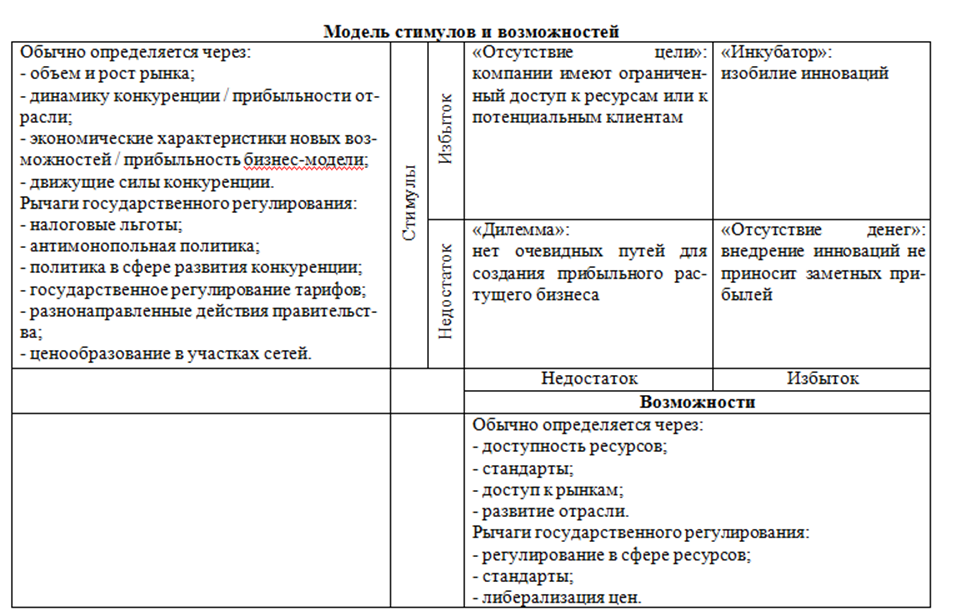
\includegraphics[scale=.45]{img/stimul_possibility_model}
\end{table}
\end{frame}
\end{document}